\documentclass[11pt,a4paper]{article}

\usepackage[margin=2.3cm]{geometry}
\usepackage[T1]{fontenc}
\usepackage{lmodern}
\usepackage{microtype}
\usepackage{amsmath,amssymb}
\usepackage{graphicx}
\usepackage{booktabs}
\usepackage{caption}
\usepackage{float}
\usepackage[hidelinks]{hyperref}
\usepackage[version=4]{mhchem}
\usepackage{siunitx}

\graphicspath{{../figures/}}
\captionsetup{font=small,labelfont=bf}
\setlength{\parskip}{3pt}

\newcommand{\CH}{\ce{CH4}}
\newcommand{\OH}{\ce{OH}}

\title{\textbf{Why Is Methane Rising Again?}\\[2pt]
\large A Methane--OH Box Model of Recent Trends\\ and the Global Methane Pledge}
\author{Shardul Junagade (23110297)\\[2pt]
\small EH-605 Modeling Earth System and Sustainability, IIT Gandhinagar\\
\small Instructor: Prof.\ R.\ N.\ Singh\\[2pt]
\small Final project report}
\date{November 2026}

\begin{document}
\maketitle

\begin{abstract}
\noindent
Atmospheric methane has been measured continuously since 1983, and its record is not a smooth curve. Growth almost stopped between 2000 and 2006, picked up again in 2007, and hit a record of about 15--18\,ppb\,yr$^{-1}$ in 2020--21. I tried to understand this record with the simplest models possible, adding detail only where the data forced me to.

A one-box model with a constant lifetime fails: with the known lifetime of about 9 years it misses the observations by 21\,ppb (RMS) and shows no stall at all. Treating the \CH--\OH\ reaction by mass action gives a stiff two-variable system. Its fast variable (\OH) relaxes in about a second, so the system reduces to a single equation with a saturating, Michaelis--Menten-like sink. This feedback stretches the lifetime of a methane perturbation from 9.3 to 12.7 years, but on its own it makes the fit worse. The fit becomes good (RMS error 3\,ppb, out-of-sample error 7\,ppb) only when \OH\ is also allowed to respond to NOx and CO emissions and to temperature. With this model, rising NOx explains part of the stall and the COVID drop in NOx explains roughly half of the 2020--21 surge. A two-hemisphere box model places the remaining, non-inventory emissions mostly in the tropics.

I then coupled the fitted model to a two-layer energy-balance model and solved a dynamic optimisation in GEKKO. Meeting the Global Methane Pledge would lower methane in 2050 by about 330\,ppb and avoid about 0.05\,K of warming through methane's direct forcing, and an economically optimal abatement level comes out close to the pledge's 30\,\%. India, which emits 9\,\% of the world's methane, emits half the world average per person, mostly from livestock and rice.
\end{abstract}

\section{Introduction}

Methane (\CH) is the second most important greenhouse gas made by people. Its concentration has risen from about 729\,ppb before industrialisation to 1936\,ppb in 2025, and its radiative forcing today is about \SI{0.57}{W.m^{-2}}, roughly a quarter of that of \ce{CO2}. Unlike \ce{CO2}, methane does not stay in the air for centuries. It is destroyed mainly by the hydroxyl radical (\OH) in the troposphere, which gives it a lifetime of about a decade. A short lifetime makes methane attractive for policy: cutting emissions should show up in the atmosphere within a few years. That idea is behind the Global Methane Pledge, signed in 2021, which aims to cut anthropogenic methane emissions by 30\,\% from 2020 levels by 2030.

The same short lifetime makes the observed record hard to read. The growth rate of methane (Fig.~\ref{fig:record}) has gone through three surprising changes:
\begin{itemize}\itemsep0pt
\item a near standstill from 2000 to 2006;
\item a restart in 2007;
\item an unusually fast rise in 2020--21, during the pandemic, when human activity dropped.
\end{itemize}
Emission inventories do not show anything like a pause in 2000--06; if anything they grow fastest then. So either the inventories are missing something, or the sink is changing. The sink is interesting in its own right because methane uses up its own destroyer. More methane means less \OH, which means methane lives longer, which is a positive feedback similar to the ice--albedo feedback in climate.

My aim was not to build a chemistry-climate model, but to see how far simple models can go on a real problem: box models and residence times, stability and feedback analysis, mass-action kinetics, energy balance and dynamic optimisation. The rule I followed throughout was to start with the simplest model and add a process only when the observations showed that the simpler model was not enough.

\begin{figure}[t]
\centering
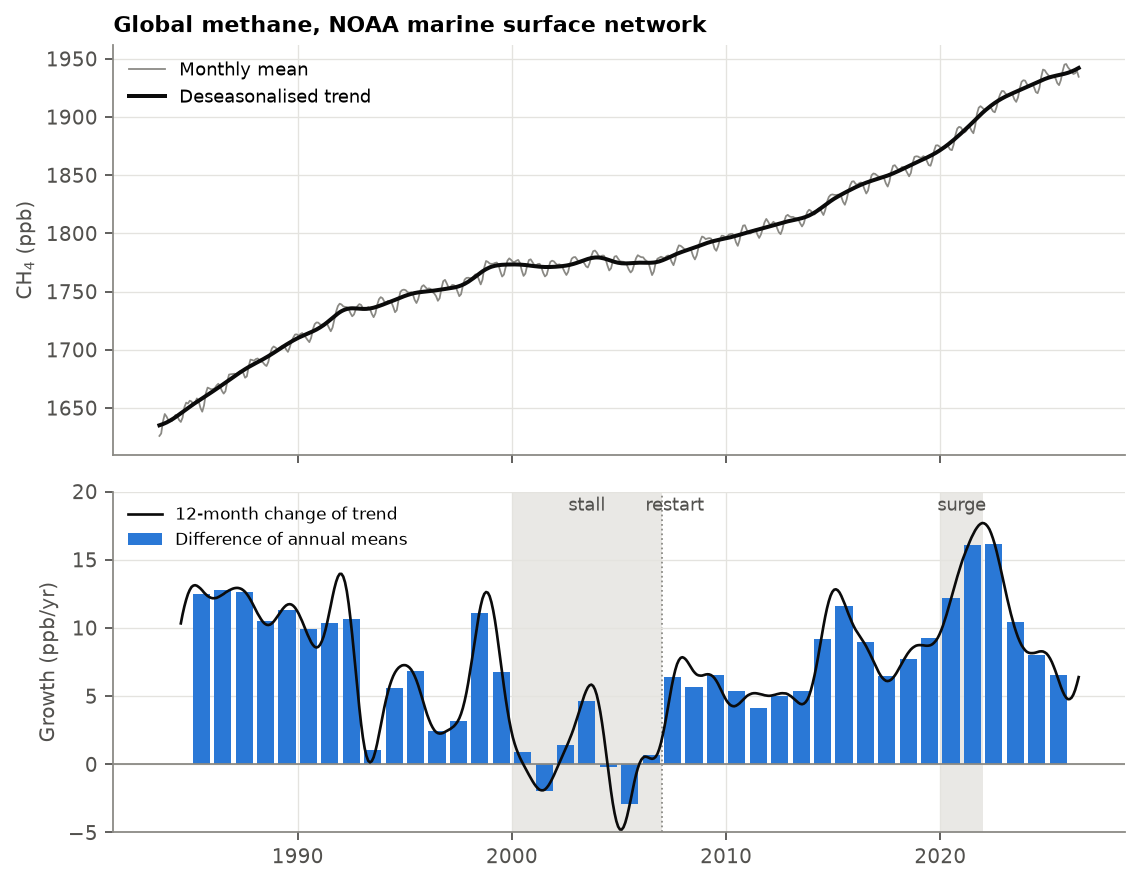
\includegraphics[width=0.82\linewidth]{01_record_growth.png}
\caption{Global mean methane from the NOAA marine surface network (top) and its growth rate (bottom). The stall, restart and surge that motivate this project are marked.}
\label{fig:record}
\end{figure}

\section{Objectives}

The project outline listed three objectives and, as expected outcomes, a model that explains the growth rate, a comparison of the pledge with an optimal path, and a look at India. In the final work these became five objectives:

\begin{enumerate}\itemsep2pt
\item \textbf{Test the one-box model.} Find out whether a one-box model with a constant lifetime can reproduce the observed methane record since 1984, and if it cannot, understand why.
\item \textbf{Analyse the methane--OH system.} Build a coupled methane--\OH\ model, study its equilibria, stability and feedback strength, and check whether it has a tipping point.
\item \textbf{Explain the observed growth rate.} Find which processes (anthropogenic emissions, the drivers of \OH, temperature) explain the stall, the restart and the 2020 surge, and where any unexplained emissions are located.
\item \textbf{Evaluate the Global Methane Pledge.} Estimate how much the pledge would lower methane concentration and warming by 2050, and compare it with an economically optimal abatement path.
\item \textbf{Look at India.} Describe India's methane emissions: their sources, their intensity per person and per unit of GDP, and what an Indian contribution to the pledge would achieve.
\end{enumerate}

\section{Data}

All data are public and were downloaded by a script that also checks each file (coverage, value ranges, and agreement between overlapping sources). The datasets are listed in Table~\ref{tab:data}.

\begin{table}[h]
\centering\small
\caption{Datasets used.}
\label{tab:data}
\begin{tabular}{p{5.3cm}p{3.2cm}p{6.1cm}}
\toprule
Dataset & Period & Used for\\
\midrule
NOAA GML global mean \CH\ (monthly, annual) & 1983--2026 & target of every model fit\\
NOAA flask \CH\ at 23 stations & 1983--2025 & north--south gradient\\
NOAA HATS methyl chloroform (NH, SH) & 1992--2025 & tracer for interhemispheric mixing\\
EDGAR 2025 \CH\ by country and sector & 1970--2024 & anthropogenic emissions, India\\
CEDS + fires (ClimateIndicator) & 1970--2025 & second inventory, NOx and CO emissions\\
ClimateIndicator concentrations and ERF & 1750--2025 & spin-up, forcing check, total forcing\\
Global Carbon Project methane budget & 2000--2020 & independent budget check\\
HadCRUT5 global temperature & 1850--2025 & energy-balance calibration\\
RCMIP SSP emissions and concentrations & to 2100 & future scenarios\\
Our World in Data (population, GDP) & 1990--2022 & India comparison\\
\bottomrule
\end{tabular}
\end{table}

A few properties of the data matter for what follows.
\begin{itemize}\itemsep0pt
\item \textbf{Inventories disagree.} EDGAR gives 333\,Tg\,yr$^{-1}$ of anthropogenic methane for 2024, while CEDS with fires gives 368. EDGAR also leaves out wildfires.
\item \textbf{Inventories grow fastest during the stall.} EDGAR grows by 3.9\,Tg\,yr$^{-2}$ during 2000--06 but only 2.8\,Tg\,yr$^{-2}$ during 2007--19, the opposite of what the concentrations do.
\item \textbf{Provisional values.} The newest NOAA months are preliminary, and the last HadCRUT year (2026) is incomplete; both are left out.
\end{itemize}
I convert between mass and mixing ratio with $\beta=\SI{2.75}{Tg}$ per ppb, the methane analogue of the 2.123\,GtC per ppm used for \ce{CO2}.

\section{Methodology}

\subsection{Overall approach}
The work proceeded in four stages.
\begin{enumerate}\itemsep0pt
\item \textbf{Simple models first.} I wrote down the simplest models (a one-box model, then the \CH--\OH\ kinetic system) and analysed them on paper: equilibria, stability, time scales.
\item \textbf{Fitting a hierarchy.} I fitted a hierarchy of increasingly detailed versions to the observed record. A new process was added only if it improved the fit and the out-of-sample prediction.
\item \textbf{Locating the emissions.} A separate two-hemisphere model was used to locate the emissions the inventory cannot explain.
\item \textbf{Applications.} The best model was used for forcing and warming, future scenarios, an optimal abatement problem and the India analysis.
\end{enumerate}


\subsection{One-box model and mass balance}
The simplest description treats the atmosphere as one well-mixed box:
\begin{equation}
\frac{dC}{dt}=\frac{E_a(t)+E_n}{\beta}-\frac{C}{\tau},
\label{eq:onebox}
\end{equation}
where $C$ is the global mean mixing ratio, $E_a$ the anthropogenic emissions from EDGAR, $E_n$ a constant natural source and $\tau$ the lifetime. For exponentially growing emissions $E_a=q\,e^{\alpha t}$ it has the closed-form solution
\begin{equation}
C(t)=C_0e^{-t/\tau}+\frac{E_n\tau}{\beta}\left(1-e^{-t/\tau}\right)+\frac{q/\beta}{\alpha+1/\tau}\left(e^{\alpha t}-e^{-t/\tau}\right),
\end{equation}
which I used to check the numerical solver. Turned around, the same equation gives the total emissions implied by the observations,
\begin{equation}
E(t)=\beta\left(\frac{dC}{dt}+\frac{C}{\tau}\right),
\label{eq:topdown}
\end{equation}
without any inventory, with $dC/dt$ from centred differences of the annual means. Finally, to test the model over a longer period, I started it in 1750 at the ice-core value of 729\,ppb and ran it forward with the historical emission series, as in the Rodhe--Bj\"orkstr\"om carbon model.

\subsection{Methane and OH as a kinetic system}
By the law of mass action, the reaction $\ce{CH4 + OH -> products}$ proceeds at a rate proportional to $[\CH][\OH]$. Writing $X$ for \OH\ relative to its 2010 value, a minimal two-variable system is
\begin{align}
\frac{dC}{dt}&=\frac{E}{\beta}-k\,X\,C-k_oC, \label{eq:ch4}\\
\frac{dX}{dt}&=\frac{1}{\tau_X}\Big[P-X\Big(a\frac{C}{C_r}+1-a\Big)\Big], \label{eq:oh}
\end{align}
where $P$ is the \OH\ production and the other parameters are listed in Table~\ref{tab:params}. The term in brackets says that \OH\ is destroyed partly by methane (a share $a$) and partly by other gases, mainly CO.

\OH\ lives about one second ($\tau_X\approx\SI{1}{s}$), so it settles almost at once. Setting $dX/dt=0$ gives a single equation with a saturating sink,
\begin{equation}
S(C)=\frac{k\,C}{a\,C/C_r+1-a}+k_oC,
\label{eq:sink}
\end{equation}
which has the same shape as the Michaelis--Menten (Monod) uptake law. Two lifetimes follow from it: the global lifetime $\tau=C/S(C)$ and the perturbation lifetime $\tau_p=1/S'(C)$, which controls how fast an extra pulse of methane decays (from linear stability analysis). Their ratio $f=\tau_p/\tau$ is the feedback factor. The equilibria for a given emission rate solve $E/\beta=S(C)$, and their stability follows from the Jacobian of Eqs.~\eqref{eq:ch4}--\eqref{eq:oh}.

\begin{table}[t]
\centering\small
\caption{Model parameters. ``Fitted'' values are from the best model (V4) with one standard error.}
\label{tab:params}
\begin{tabular}{llll}
\toprule
Symbol & Meaning & Value & Source\\
\midrule
$\beta$ & Tg of \CH\ per ppb & 2.75 & GCP convention\\
$1/k$ & \CH\ lifetime against \OH\ (prior) & $11.2\pm1.3$\,yr & Prather et al.\ (2012)\\
$k$ & \OH\ loss frequency of \CH & $0.098\pm0.004$\,yr$^{-1}$ & fitted\\
$k_o$ & stratosphere, soil and Cl sinks & 0.020\,yr$^{-1}$ & Prather et al.\ (2012)\\
$a$ & share of \OH\ loss due to \CH & 0.31 & Holmes et al.\ (2013)\\
$C_r$ & reference \CH\ (2010) & 1799\,ppb & NOAA\\
$E_n$ & natural + non-inventory source & $306\pm19$\,Tg\,yr$^{-1}$ & fitted\\
$g_N$, $g_C$ & \OH\ sensitivity to NOx, CO emissions & $0.33\pm0.02$, $0.19\pm0.02$ & fitted\\
$E_a/R$ & activation temperature of \CH+\OH & 1775\,K & Burkholder et al.\ (2019)\\
$\tau_{ex}$ & interhemispheric exchange time & $1.03\pm0.09$\,yr & fitted (methyl chloroform)\\
$C$ & upper-layer heat capacity & 16.7\,W\,yr\,m$^{-2}$\,K$^{-1}$ & fitted (HadCRUT5)\\
$\lambda$ & climate feedback parameter & 1.25\,W\,m$^{-2}$\,K$^{-1}$ & fitted (HadCRUT5)\\
$\gamma$ & deep-ocean coupling & 0.67\,W\,m$^{-2}$\,K$^{-1}$ & Geoffroy et al.\ (2013)\\
$C_d$ & deep-ocean heat capacity & 100\,W\,yr\,m$^{-2}$\,K$^{-1}$ & Geoffroy et al.\ (2013)\\
\bottomrule
\end{tabular}
\end{table}

\subsection{Model hierarchy, fitting and evaluation}
I fitted increasingly detailed versions of Eq.~\eqref{eq:ch4}, with \OH\ in steady state, to the NOAA annual means for 1984--2025.
\begin{itemize}\itemsep0pt
\item \textbf{V1:} constant lifetime (Eq.~\ref{eq:onebox}).
\item \textbf{V2:} adds the \CH--\OH\ feedback (Eq.~\ref{eq:sink}).
\item \textbf{V3:} also lets \OH\ production depend on NOx and CO emissions:
\[P=\left(\frac{E_{\mathrm{NOx}}}{E_{\mathrm{NOx},r}}\right)^{g_N}\left(\frac{E_{\mathrm{CO}}}{E_{\mathrm{CO},r}}\right)^{-g_C}.\]
\item \textbf{V4:} additionally lets the rate constant follow the Arrhenius law with the observed temperature anomaly, $k\propto \exp(1775\,\Delta T/T^2)$ with $T=272$\,K.
\end{itemize}

The parameters $\theta$ were found by minimising
\begin{equation}
J(\theta)=\sum_{i}\left(\frac{C_{\mathrm{model},i}-C_{\mathrm{obs},i}}{\sigma}\right)^2+\left(\frac{k-k_0}{\sigma_k}\right)^2,
\end{equation}
with $\sigma=3$\,ppb.

The second term needs a word of explanation. The lifetime and the natural source turned out to trade off against each other (Section~\ref{sec:onebox}), so the data alone cannot fix both. I therefore added the literature value $1/k_0=11.2\pm1.3$\,yr as a soft constraint. Parameter standard errors come from the Jacobian of the residuals at the optimum.

Models were compared in three ways:
\begin{itemize}\itemsep0pt
\item by the RMS error;
\item by the Akaike information criterion, $\mathrm{AIC}=n\ln(\mathrm{RSS}/n)+2p$, which penalises extra parameters;
\item by a holdout test: fit to 1984--2012 only, then predict 2013--2025.
\end{itemize}
To attribute the three events, I re-ran the best model with one driver (anthropogenic emissions, NOx, CO or temperature) held at its value from the year before the event, and measured how much the mean growth rate changed.

\subsection{Two-hemisphere model}
The northern and southern hemispheres form two boxes that exchange air on a time scale $\tau_{ex}$, the same structure as two-box carbon-cycle models:
\begin{equation}
\frac{dN}{dt}=\frac{2fE}{\beta}-\frac{N}{\tau}-\frac{N-S}{\tau_{ex}},\qquad
\frac{dS}{dt}=\frac{2(1-f)E}{\beta}-\frac{S}{\tau}+\frac{N-S}{\tau_{ex}},
\label{eq:hemi}
\end{equation}
with $f$ the fraction of emissions in the north.

I first fitted the same model to methyl chloroform for 1993--2015, to get $\tau_{ex}$. Methyl chloroform is an industrial solvent emitted almost entirely in the north, so I assumed $f=0.98$. With $\tau_{ex}$ known, the observed methane gradient $N-S$ gives $f$ for methane year by year. Hemispheric means were built from the 23 stations (leaving out two mountain stations) by interpolating in $\sin(\text{latitude})$, which weights each latitude by its area.

\subsection{Forcing and warming}
Methane forcing was computed with the simple square-root formula $0.036(\sqrt{M}-\sqrt{M_0})$ and with two published versions (Myhre et al., 1998; Etminan et al., 2016), and compared with the official series. Warming was computed with a zero-dimensional energy-balance model extended by a deep-ocean layer, that is, a two-box model for heat:
\begin{equation}
C\frac{dT}{dt}=F-\lambda T-\gamma(T-T_d),\qquad C_d\frac{dT_d}{dt}=\gamma(T-T_d).
\label{eq:ebm}
\end{equation}
$C$ and $\lambda$ were fitted to the HadCRUT5 anomalies (relative to 1850--1900) using the total forcing from 1750. The deep-ocean values $\gamma$ and $C_d$ were taken from the literature. For comparison I also fitted the one-layer model ($\gamma=0$).

\subsection{Scenarios, uncertainty and the climate feedback loop}
For the future, the best model was driven by:
\begin{itemize}\itemsep0pt
\item the SSP scenarios (their methane, NOx and CO emissions relative to 2025, and the IPCC AR6 warming of each scenario);
\item the pledge path, a linear cut to 70\,\% of the 2020 level by 2030, then held;
\item two limiting cases: emissions frozen at 2025, and emissions stopped entirely.
\end{itemize}
Warming differences between scenarios were computed with Eq.~\eqref{eq:ebm}. Uncertainty in the pledge result was estimated from 200 Monte Carlo runs. Each run drew the fitted parameters from their covariance, $a$ from 0.25--0.37 and $\lambda$ from $1.25\pm0.25$.

To ask whether warming could set off a methane runaway through wetlands, I computed the gain of the closed loop warming $\to$ wetland emissions $\to$ methane $\to$ forcing $\to$ warming, using standard feedback analysis:
\begin{equation}
g=\frac{dT}{dF}\cdot\frac{dF}{dC}\cdot\frac{dC^*}{dE}\cdot\frac{dE}{dT}.
\label{eq:gain}
\end{equation}
A gain of 1 means a runaway. Wetland emissions (165\,Tg\,yr$^{-1}$, from the Global Carbon Project) were assumed to grow by a factor $Q_{10}$ per 10\,K of warming, and $Q_{10}$ was varied from 1 to 4.

\subsection{Optimal abatement}
As in the classic optimal fishery-harvest problem, I posed abatement as an optimal-control problem. The control $u(t)\in[0,0.7]$ is the fraction of baseline (SSP2-4.5) anthropogenic emissions removed. Abatement costs $\tfrac12 m u^2E_b$ per year, with $m=\$4000$\,t$^{-1}$, so that the marginal cost rises linearly with $u$. Two problems were solved.

\textbf{Problem A} weighs abatement costs against climate damage:
\begin{equation}
\min_u\ \sum_t e^{-rt}\Big[\tfrac12 m\,u^2E_b+D\,C\Big],\qquad r=2\,\%\,\text{yr}^{-1},
\end{equation}
where $D$ is chosen so that one tonne emitted today costs the social cost of methane (\$800, \$1600 or \$3200 per tonne).

\textbf{Problem B} finds the cheapest path that reaches the pledge's 2050 concentration and stays below it afterwards.

\subsection{India}
India's emissions by sector come from EDGAR, and population and GDP from Our World in Data. To separate the causes of emission growth between 1990 and 2022, I used the identity
\begin{equation}
E=P\times\frac{G}{P}\times\frac{E}{G},
\end{equation}
emissions = population $\times$ income per person $\times$ methane per unit of GDP, a Kaya-type decomposition. The effect of a 30\,\% Indian cut was simulated with the best model on top of SSP2-4.5.

\subsection{Numerical implementation}
Everything was written in Python.
\begin{itemize}\itemsep0pt
\item \textbf{Box models.} These were integrated with a fourth-order Runge--Kutta scheme with monthly steps and annually constant emissions. Against the analytic solution, the error is 0.08\,ppb.
\item \textbf{Stiff system.} The full two-variable \CH--\OH\ system was solved with an implicit (Radau) solver, to check the steady-state reduction.
\item \textbf{Fits.} These used SciPy's \texttt{least\_squares}.
\item \textbf{Optimisation.} The optimal-control problems were solved with GEKKO (IMODE 6, the IPOPT solver) on an annual grid from 2025 to 2100.
\end{itemize}
The analysis is split into nine scripts that run in about two minutes.

\section{Analysis and results}

\subsection{A constant lifetime cannot explain the record}
\label{sec:onebox}
With the lifetime fixed at 9.15\,yr, the one-box model misses the observations by 21\,ppb RMS (Fig.~\ref{fig:onebox}). Worse, it has no stall: it keeps growing through 2000--06, because EDGAR emissions keep growing. When the model is fitted only to 1984--2005 and run forward, it overshoots 2025 by 39\,ppb. If the lifetime is left free, the fit improves to 12.6\,ppb, but only by shrinking the lifetime to 6.4\,yr and pushing the natural source to 500\,Tg\,yr$^{-1}$. Both are physically unrealistic.

The misfit surface explains why. The error has a long, narrow valley along which a shorter lifetime is traded for a larger natural source, so the data alone cannot pin down both. This is the reason the later fits carry a prior on the lifetime.

\begin{figure}[t]
\centering
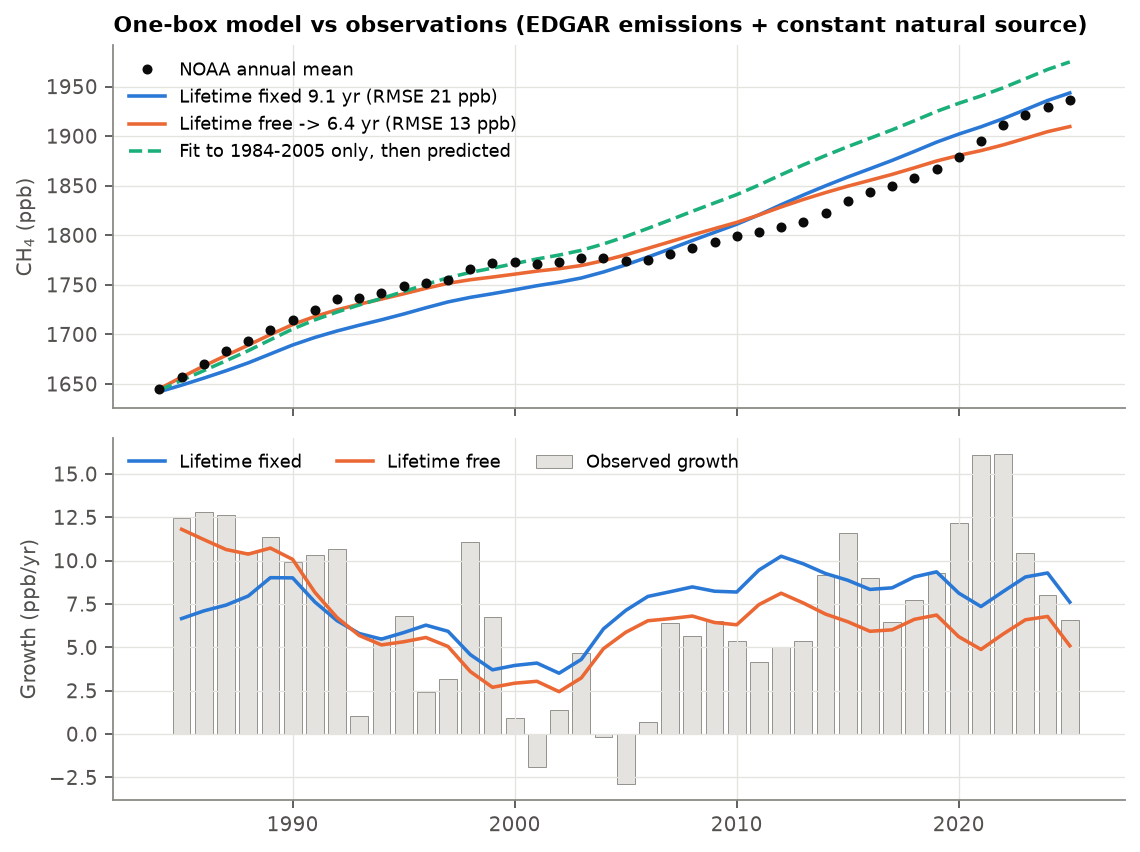
\includegraphics[width=0.56\linewidth]{02_one_box_fit.png}\hfill
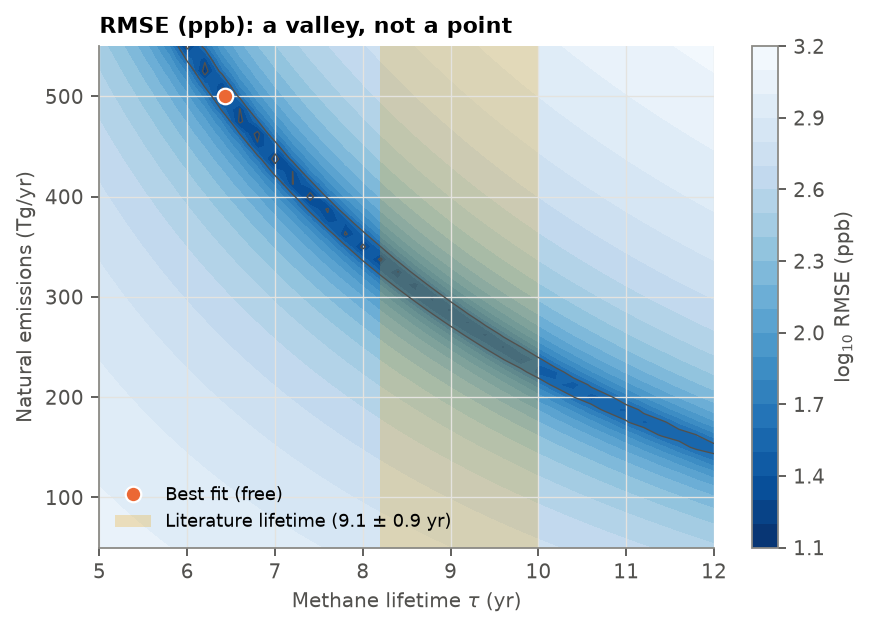
\includegraphics[width=0.42\linewidth]{02_cost_surface.png}
\caption{Left: the one-box model against observations, with fixed and free lifetime, and a run fitted only to 1984--2005. Right: RMS error as a function of lifetime and natural emissions. The minimum is a valley, not a point; the yellow band is the lifetime known from independent studies.}
\label{fig:onebox}
\end{figure}

Using the same equation the other way round (Eq.~\ref{eq:topdown}) is more useful. With $\tau=9.1$\,yr, the observed record implies total emissions of 574\,Tg\,yr$^{-1}$ for 2010--19. That is almost identical to the Global Carbon Project's independent estimate of 575\,Tg\,yr$^{-1}$ (Fig.~\ref{fig:topdown}, left). The part not covered by EDGAR (natural sources plus whatever the inventory misses) behaves as follows:

\begin{center}\small
\begin{tabular}{lccccc}
\toprule
Period & 1985--99 & 2000--06 & 2007--19 & 2020--22 & 2023--24\\
\midrule
Non-EDGAR emissions (Tg\,yr$^{-1}$) & 289 & 268 & 267 & 291 & 273\\
\bottomrule
\end{tabular}
\end{center}

\noindent It dropped by about 20\,Tg\,yr$^{-1}$ during the stall and rose by about 25 in the surge.

The spin-up from 1750 (Fig.~\ref{fig:topdown}, right) adds a longer view. A natural source that keeps the pre-industrial 729\,ppb in balance (219\,Tg\,yr$^{-1}$) gives the right concentration in 1850 but only 1760\,ppb in 2025. The natural source fitted to 1984--2025 (274\,Tg\,yr$^{-1}$) matches today but is far too high before 1950. So the emissions missing from the inventory today are about 55\,Tg\,yr$^{-1}$ larger than the pre-industrial natural source. This is either sources the inventory leaves out or natural emissions that have grown.

\begin{figure}[t]
\centering
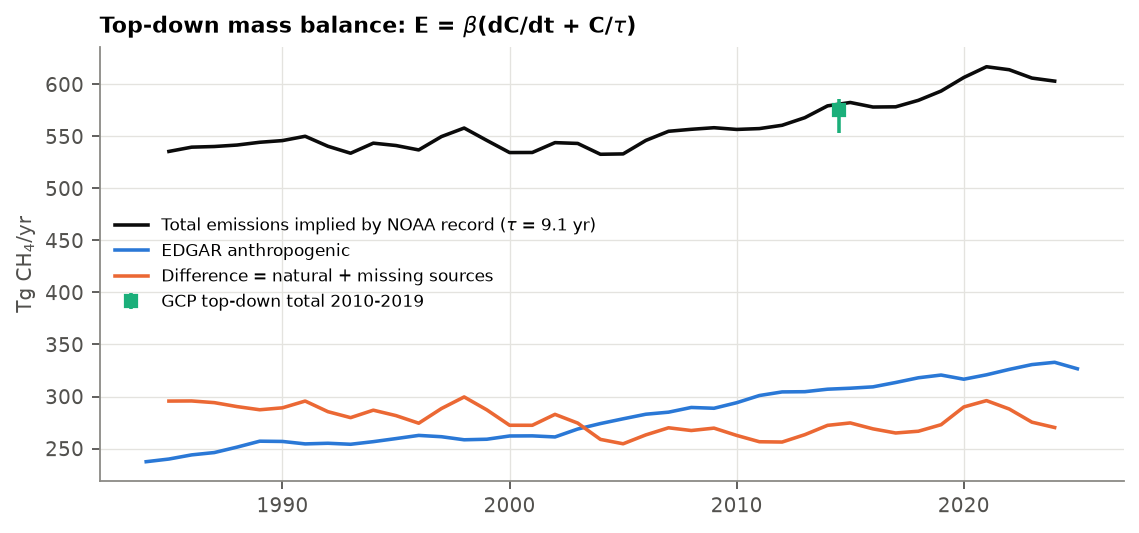
\includegraphics[width=0.5\linewidth]{02_topdown_emissions.png}\hfill
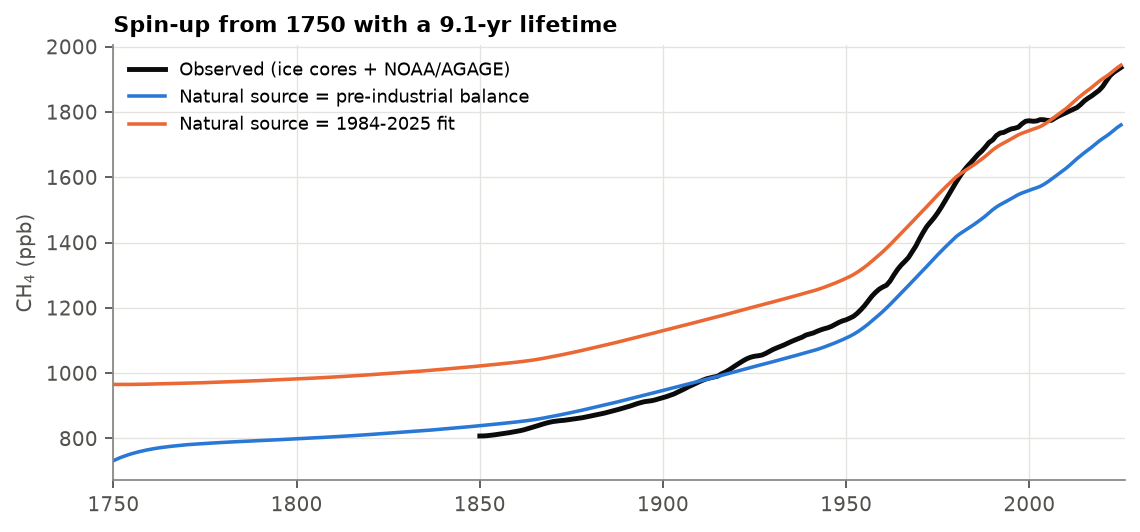
\includegraphics[width=0.48\linewidth]{02_spinup_1750.png}
\caption{Left: total emissions implied by the observed record (Eq.~\ref{eq:topdown}), EDGAR anthropogenic emissions and their difference, with the Global Carbon Project estimate for 2010--19. Right: one-box model started in 1750 with two choices of natural source, against ice-core and instrumental methane.}
\label{fig:topdown}
\end{figure}

\subsection{The methane--OH feedback}
At today's state, the Jacobian of Eqs.~\eqref{eq:ch4}--\eqref{eq:oh} has two eigenvalues:
\begin{itemize}\itemsep0pt
\item $-3.2\times10^{7}$\,yr$^{-1}$, a time scale of 0.98\,s, for \OH;
\item $-0.079$\,yr$^{-1}$, a time scale of 12.7\,yr, for methane.
\end{itemize}
The system is extremely stiff, and replacing it by the reduced Eq.~\eqref{eq:sink} changes the solution by only $4\times10^{-6}$\,ppb. The phase portrait (Fig.~\ref{fig:oh}, right) shows this fast--slow structure directly: trajectories drop almost vertically onto the \OH\ nullcline and then creep along it towards a single stable node.

The feedback lengthens the response time. In 2025 the global lifetime is 9.33\,yr but the perturbation lifetime is 12.69\,yr. That is a feedback factor of $f=1.36$, inside the 1.3--1.4 range quoted in the literature. A 100\,Tg pulse decays with an e-folding time of 12.7\,yr with feedback and 9.2\,yr without, consistent with the eigenvalue. Methane itself has already lowered \OH\ by about 2\,\% since 2010.

\begin{figure}[t]
\centering
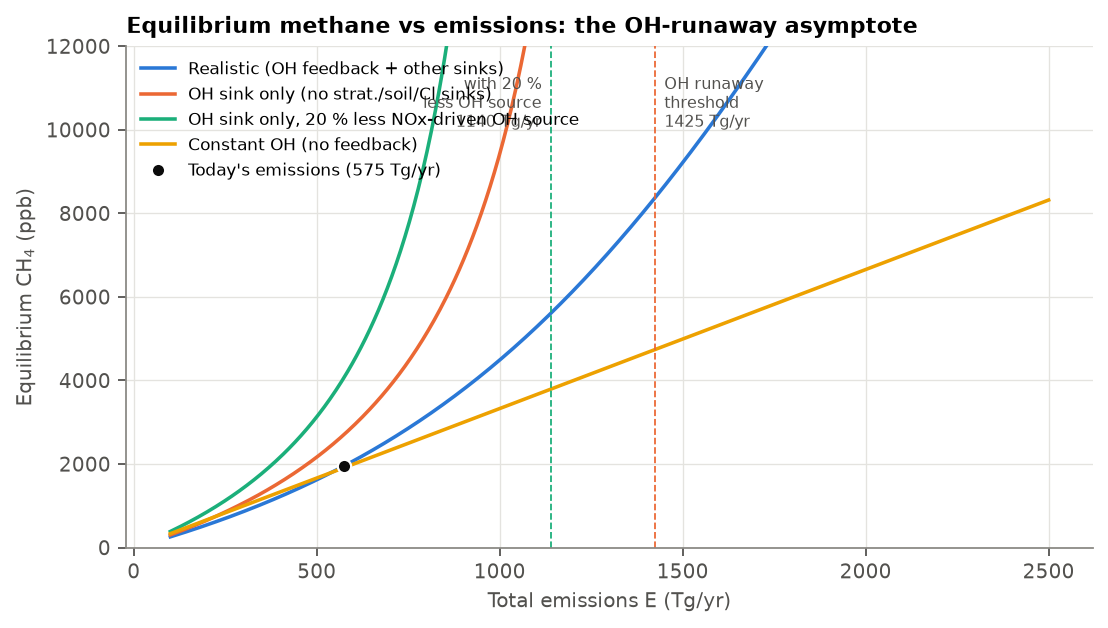
\includegraphics[width=0.49\linewidth]{03_equilibrium_threshold.png}\hfill
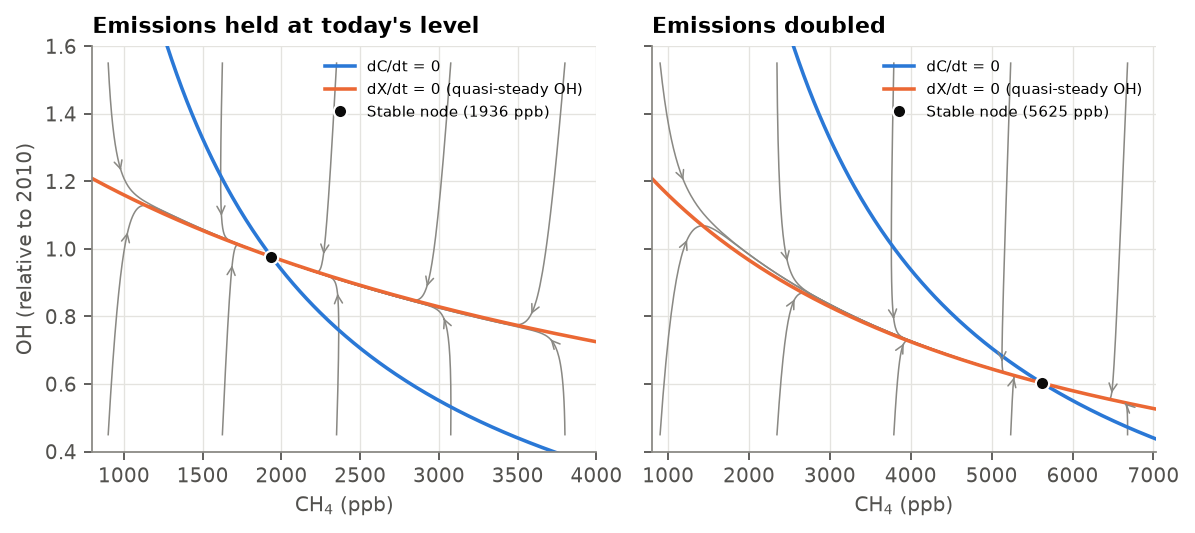
\includegraphics[width=0.49\linewidth]{03_phase_portrait.png}
\caption{Left: equilibrium methane as a function of total emissions. With \OH\ as the only sink, equilibrium is lost at 1425\,Tg\,yr$^{-1}$ (dashed); the other sinks remove this asymptote. Right: phase portraits for today's emissions and for doubled emissions (\OH\ slowed artificially to make the fast step visible).}
\label{fig:oh}
\end{figure}

Is there a tipping point? Because $S(C)$ increases monotonically, there is exactly one stable equilibrium for any emission rate. There is no bistability and no hysteresis, unlike the snowball-Earth energy-balance model.

If \OH\ were the only sink, though, the saturation in Eq.~\eqref{eq:sink} would cap removal at $\beta kC_r/a$. Above
\begin{equation}
E_{\mathrm{crit}}=\frac{\beta\,k\,C_r}{a}\approx\SI{1425}{Tg.yr^{-1}}
\end{equation}
no equilibrium would exist at all. That is about 2.5 times today's emissions, and it drops to 1140\,Tg\,yr$^{-1}$ if the \OH\ source falls by 20\,\%. The slower, non-saturating sinks ($k_oC$) remove the singularity. Equilibrium methane then rises steeply with emissions but stays finite. Holding today's 575\,Tg\,yr$^{-1}$ forever would bring methane to about 1955\,ppb, only slightly above today's level.

\subsection{What explains the stall, restart and surge}
Table~\ref{tab:models} and Fig.~\ref{fig:fits} compare the model hierarchy.

The first surprise was that adding the \CH--\OH\ feedback on its own (V2) makes the fit worse, not better (RMS error 32\,ppb against 21). The feedback amplifies the response to rising emissions, so it pushes the model even further away from a stall. What fixes the fit is letting \OH\ respond to things outside the methane cycle. With NOx and CO emissions as drivers (V3) the error drops to 3.1\,ppb. With the temperature dependence of the rate constant added (V4) the AIC is lowest, and V4 also predicts the held-out years 2013--25 best (6.7\,ppb).

The fitted sensitivities are $g_N=0.33\pm0.02$ and $g_C=0.19\pm0.02$. The value of $g_N$ is probably larger than a chemistry model would give, so I read it as an effective sensitivity that may also absorb other trends correlated with NOx. Swapping EDGAR for the CEDS inventory changes the error by less than 0.3\,ppb. Fitting the feedback strength $a$ as well, instead of fixing it, gives $0.07\pm0.14$. The concentration record cannot determine it, which is why the literature value is used.

\begin{table}[t]
\centering\small
\caption{Model hierarchy fitted to NOAA annual means, 1984--2025. ``Growth $r$'' is the correlation of modelled and observed annual growth; ``holdout'' is the RMS error for 2013--25 when fitted to 1984--2012 only.}
\label{tab:models}
\setlength{\tabcolsep}{4.5pt}
\begin{tabular}{lcccccc}
\toprule
Model & Params & $\tau$ (yr) & RMS (ppb) & AIC & Growth $r$ & Holdout (ppb)\\
\midrule
V1 one-box, lifetime fixed & 1 & 9.15 & 21.0 & 257.8 & 0.37 & 34.7\\
V1$'$ one-box, lifetime free & 2 & 6.43 & 12.6 & 216.8 & 0.48 & 17.6\\
V2 + \CH--\OH\ feedback & 1 & 9.15 & 32.2 & 293.5 & 0.20 & 62.6\\
V3 + NOx and CO drivers & 4 & 7.59 & 3.1 & 102.9 & 0.79 & 14.2\\
\textbf{V4 + Arrhenius temperature} & 4 & \textbf{8.47} & \textbf{3.0} & \textbf{100.1} & \textbf{0.80} & \textbf{6.7}\\
\bottomrule
\end{tabular}
\end{table}

\begin{figure}[t]
\centering
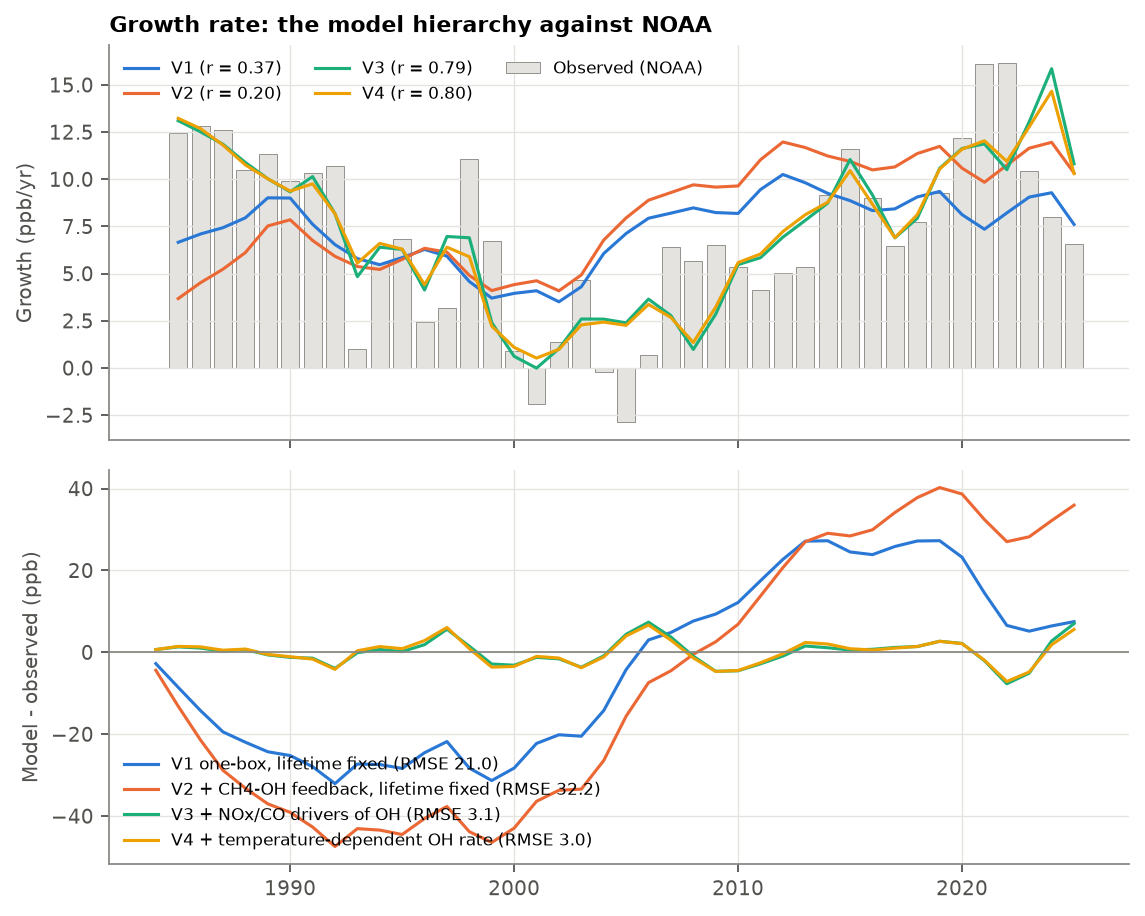
\includegraphics[width=0.55\linewidth]{04_model_hierarchy.png}\hfill
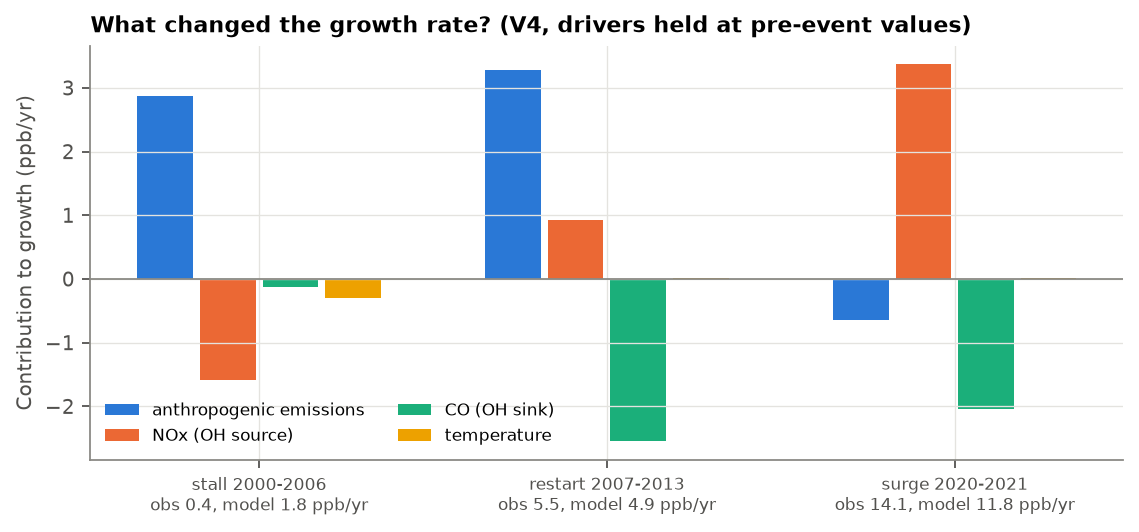
\includegraphics[width=0.44\linewidth]{04_attribution.png}
\caption{Left: modelled and observed growth rates (top) and residuals (bottom) for the model hierarchy. Right: contribution of each driver to the growth rate in the three periods, from runs with that driver held at its pre-event value.}
\label{fig:fits}
\end{figure}

Holding one driver fixed at a time (Fig.~\ref{fig:fits}, right) gives the following picture.
\begin{itemize}\itemsep0pt
\item \textbf{Stall (2000--06).} Inventory growth alone would have added about 2.9\,ppb\,yr$^{-1}$. Model \OH\ was about 3\,\% higher than in the late 1990s, mostly because NOx emissions rose, and this removed 1.6\,ppb\,yr$^{-1}$. The model still gives 1.8\,ppb\,yr$^{-1}$ against the observed 0.4. Together with the dip in non-inventory emissions found above, this suggests that natural or unaccounted emissions also fell during the stall.
\item \textbf{Restart (2007--13).} NOx emissions peaked around 2006 and \OH\ stopped rising, while emissions kept growing.
\item \textbf{Surge (2020--21).} The pandemic drop in NOx added 3.4\,ppb\,yr$^{-1}$, and lower CO emissions took away 2.0\,ppb\,yr$^{-1}$; model \OH\ fell by about 1\,\% from 2019 to 2020. The model reaches 11.8\,ppb\,yr$^{-1}$ against the observed 14.1, and the remaining gap fits the extra 25\,Tg\,yr$^{-1}$ found in the mass balance.
\end{itemize}

The surge result can be checked against an independent study. Stevenson et al.\ (2022) used sensitivities from full chemistry models and found that the lockdown cut in NOx raised methane growth by 4.8\,ppb\,yr$^{-1}$ and the cut in CO lowered it by 1.4\,ppb\,yr$^{-1}$. They concluded that these changes explain over half of the 2020 increase. My box model gives the same signs and similar sizes, which is reassuring given how simple it is.

\subsection{Where the extra methane is emitted}
The methyl chloroform fit gives an interhemispheric exchange time of $\tau_{ex}=1.03\pm0.09$\,yr, close to the textbook value of about one year. The station-based global mean agrees with NOAA's to within 0.3\,ppb on average. With this exchange time, the methane gradient of 80--95\,ppb implies that about 71--73\,\% of all methane is emitted in the north (Fig.~\ref{fig:hemi}).

EDGAR puts 82--86\,\% of anthropogenic emissions there. The rest must therefore come from sources that are only about 60\,\% northern. That points to the tropics, where large wetlands sit on both sides of the equator.

\begin{figure}[t]
\centering
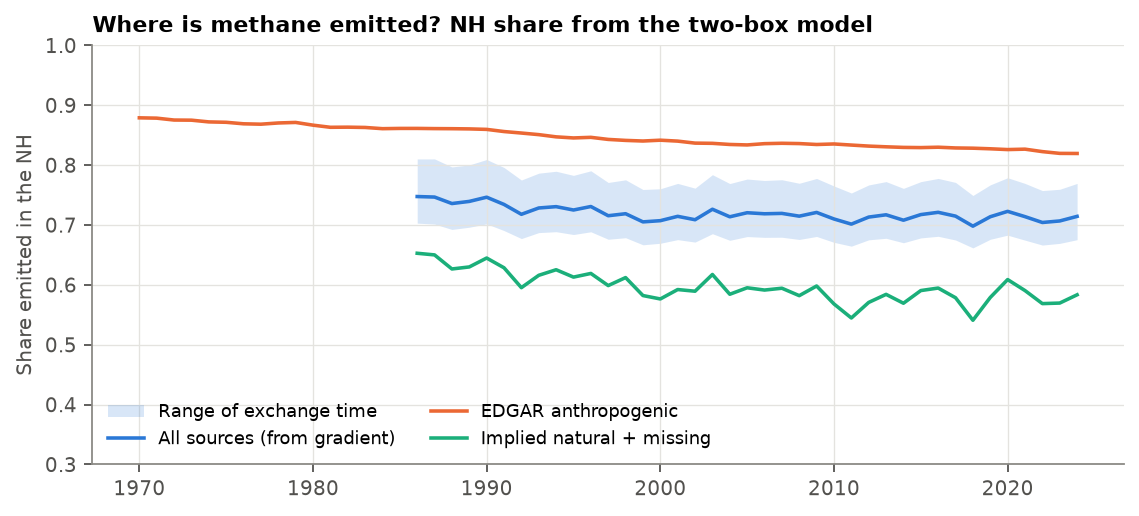
\includegraphics[width=0.62\linewidth]{05_nh_share.png}
\caption{Share of methane emitted in the northern hemisphere, from the two-box model, compared with the EDGAR inventory. The shaded band covers the uncertainty in the exchange time.}
\label{fig:hemi}
\end{figure}

\subsection{Forcing and warming}
The square-root formula gives 0.61\,W\,m$^{-2}$ for 2025, about 7\,\% above the official 0.57\,W\,m$^{-2}$, because it ignores the overlap between methane and \ce{N2O} absorption bands. The Etminan et al.\ (2016) formula with the AR6 adjustment matches the official series to 0.002\,W\,m$^{-2}$ over 1750--2025.

The one-layer energy-balance model fits HadCRUT5 with $\lambda=1.78$\,W\,m$^{-2}$\,K$^{-1}$, which implies a climate sensitivity of only 2.2\,K. It overestimates $\lambda$ because it treats heat taken up by the deep ocean as if it were a radiative feedback. With the deep-ocean layer of Eq.~\eqref{eq:ebm}, the fit gives $\lambda=1.25$\,W\,m$^{-2}$\,K$^{-1}$, close to the commonly used Budyko value $B=1.3$, and an equilibrium sensitivity of 3.1\,K (Fig.~\ref{fig:ebm}). The model warms by 1.50\,K by 2025 (observed 1.43\,K). Methane's direct forcing is responsible for 0.28\,K of this, about a fifth.

\begin{figure}[t]
\centering
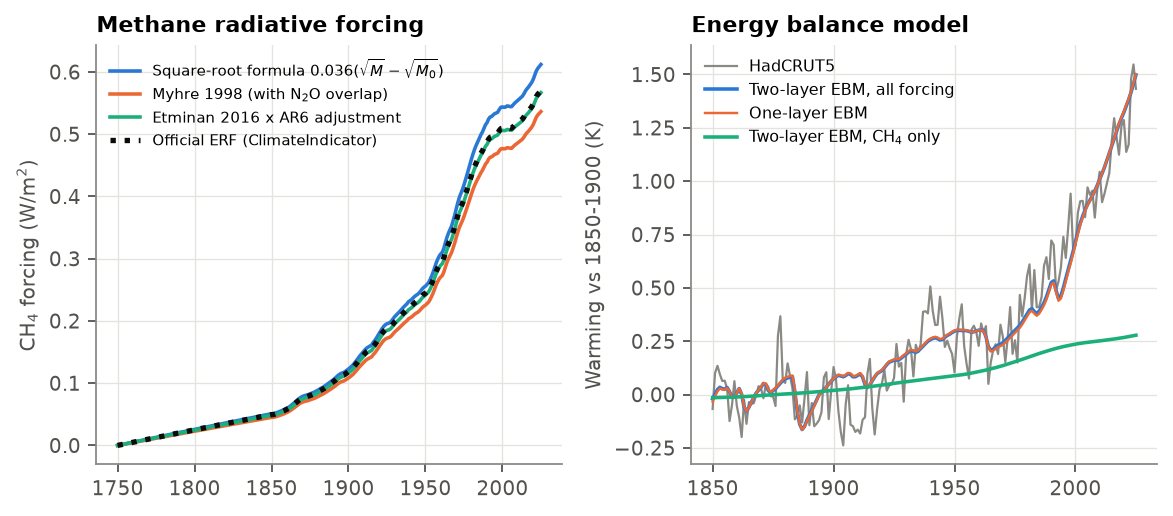
\includegraphics[width=0.85\linewidth]{06_forcing_ebm.png}
\caption{Left: methane forcing from three formulas against the official series. Right: one- and two-layer energy-balance models against HadCRUT5, and the warming due to methane alone.}
\label{fig:ebm}
\end{figure}

\subsection{Futures and the Global Methane Pledge}
Driven by the SSP scenarios, the model gives the methane paths in Fig.~\ref{fig:scen} and Table~\ref{tab:scen}. Its SSP2-4.5 projection (2005\,ppb in 2050, 1759\,ppb in 2100) is close to that of MAGICC7, the emulator used in IPCC assessments (2020 and 1683\,ppb). If all anthropogenic emissions stopped, methane would decay with an e-folding time of 9.9\,yr towards about 835\,ppb.

The pledge lowers methane in 2050 by 333\,ppb (5--95\,\% range 310--352) compared with SSP2-4.5, and avoids 0.055\,K (0.047--0.065\,K) of warming through methane's direct forcing. The pledge's own claim of at least 0.2\,K by 2050 is larger, mainly because it counts methane's indirect effects through ozone and other routes, which this model leaves out. Because methane lives about a decade, the benefit appears quickly but disappears just as quickly if the cuts are not maintained.

\begin{table}[h]
\centering\small
\caption{Methane (ppb) and warming relative to SSP2-4.5 for selected futures.}
\label{tab:scen}
\begin{tabular}{lcccc}
\toprule
Scenario & 2030 & 2050 & 2100 & $\Delta T_{2050}$ (K)\\
\midrule
SSP1-1.9 & 1943 & 1860 & 1651 & $-0.022$\\
SSP2-4.5 (baseline) & 1978 & 2005 & 1759 & 0\\
SSP3-7.0 & 1988 & 2222 & 2958 & $+0.022$\\
SSP5-8.5 & 1983 & 2266 & 2304 & $+0.026$\\
Global Methane Pledge & 1891 & 1674 & 1639 & $-0.054$\\
Emissions frozen at 2025 & 1974 & 2061 & 2095 & $+0.004$\\
All anthropogenic emissions stop & 1532 & 910 & 835 & $-0.206$\\
\bottomrule
\end{tabular}
\end{table}

\begin{figure}[t]
\centering
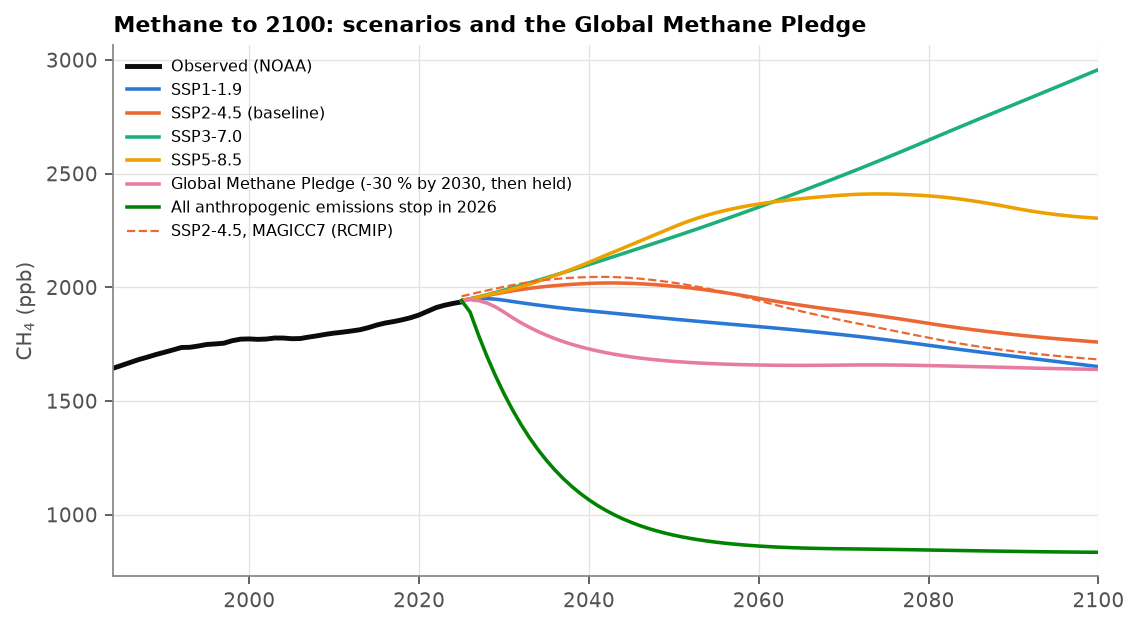
\includegraphics[width=0.56\linewidth]{07_scenarios.png}\hfill
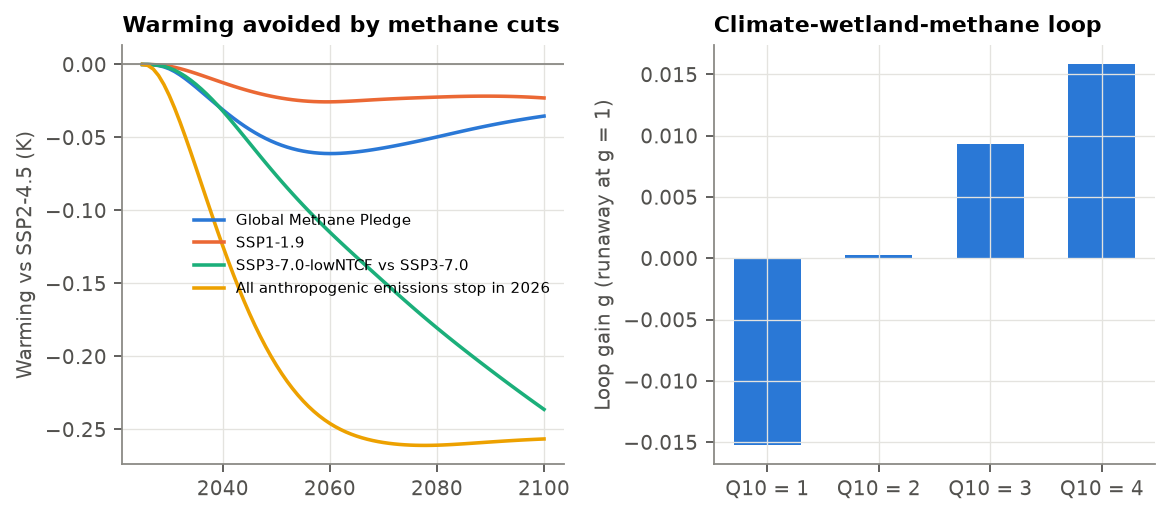
\includegraphics[width=0.43\linewidth]{07_pledge_feedback.png}
\caption{Left: projected methane for several scenarios, with the MAGICC7 projection for SSP2-4.5 (dashed). Right: warming avoided relative to SSP2-4.5, and the gain of the climate--wetland--methane loop for different wetland temperature sensitivities.}
\label{fig:scen}
\end{figure}

For the climate--wetland loop of Eq.~\eqref{eq:gain}, the first three factors are 0.80\,K per W\,m$^{-2}$, $3.7\times10^{-4}$\,W\,m$^{-2}$ per ppb and 4.6\,ppb per Tg\,yr$^{-1}$. The last factor combines the wetland response with the faster \CH--\OH\ reaction in a warmer climate, which works in the opposite direction (about $-11$\,Tg\,yr$^{-1}$ per K).

Even with a strong $Q_{10}=4$, $g$ is only 0.016. A runaway ($g=1$) would require emissions to rise by more than 700\,Tg\,yr$^{-1}$ per kelvin. This does not mean wetlands are harmless: warming caused mainly by \ce{CO2} could still add 200--350\,ppb by 2100 under SSP5-8.5 for $Q_{10}=2$--3. The response is large, but the self-amplification is small.

\subsection{Optimal abatement}
In the cost--benefit problem (Fig.~\ref{fig:opt}), GEKKO finds a nearly constant abatement fraction, set where the marginal abatement cost equals the damage caused by one more tonne. For a social cost of methane of \$800, \$1600 and \$3200 per tonne, the 2030 abatement is 19, 36 and 68\,\%, close to the analytic values of 20, 40 and 70\,\%. Abatement drops to zero at the end of the horizon, where cuts no longer have time to pay off. This is the same end effect seen in optimal fishery-harvest problems. At \$1600\,t$^{-1}$, close to the central US EPA (2023) estimate, the optimum (about 35\,\%) is close to the pledge's 30\,\%.

The target problem behaves differently. To reach the pledge's 2050 concentration as cheaply as possible, the optimiser delays: it abates 7\,\% in 2030 and builds up to a spike of 54\,\% just before 2050. Early cuts would have mostly decayed by the deadline, and later spending is discounted. The pledge path costs 1.5 times as much for the same 2050 level, but it keeps methane lower throughout the 2030s and 2040s. A target set for a single date rewards last-minute action, which is a good argument for judging methane policy by its cumulative effect rather than by an end-point.

\begin{figure}[t]
\centering
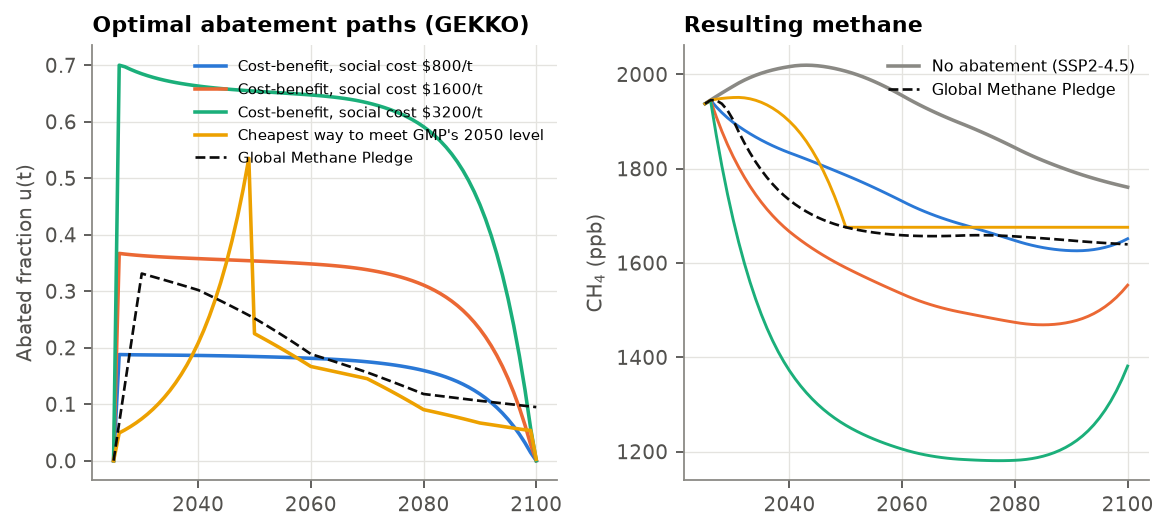
\includegraphics[width=0.85\linewidth]{08_optimal_abatement.png}
\caption{Optimal abatement paths from GEKKO for three values of the social cost of methane and for the cheapest path to the pledge's 2050 level, compared with the pledge (left), and the resulting methane (right).}
\label{fig:opt}
\end{figure}

\subsection{India}
India emitted 30.5\,Tg of methane in 2024, about 9\,\% of the world total and second only to China (51\,Tg). Two-thirds of it comes from livestock and rice, sources that are much harder to cut than leaks from oil and gas. Per person, India emits 20\,kg\,yr$^{-1}$, half the world average and a quarter of the United States (Fig.~\ref{fig:india}).

Between 1990 and 2022 India's emissions rose by 33\,\%. In the decomposition, population grew by 65\,\% and income per person by 263\,\%, while methane per unit of GDP fell by 78\,\%. India's economy has become far less methane-intensive; emissions grew because the population and incomes grew faster. A 30\,\% cut by India would be 8.4\,Tg\,yr$^{-1}$, about 9\,\% of the global pledge, and would lower 2050 methane by 32\,ppb.

\begin{figure}[t]
\centering
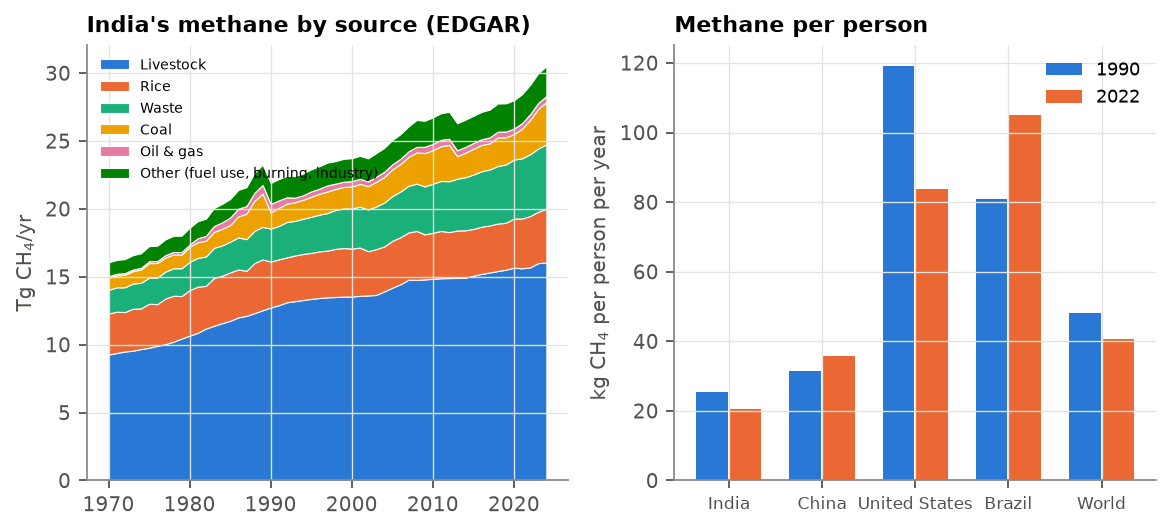
\includegraphics[width=0.8\linewidth]{09_india.png}
\caption{India's methane emissions by source (EDGAR) and methane emissions per person for selected countries in 1990 and 2022.}
\label{fig:india}
\end{figure}

\section{Limitations}
The models are deliberately simple, and several limits should be kept in mind.
\begin{itemize}\itemsep0pt
\item \textbf{One global box with annual means.} There is no seasonal cycle and no spatial structure in \OH, and the CO--\OH\ chemistry enters only through an effective exponent.
\item \textbf{Constant natural emissions.} Real wetland emissions vary with rainfall and El Ni\~no, which is why the model under-predicts the 2020--22 surge. The mass balance tells us how much extra methane there was and roughly where, but not which kind of source produced it.
\item \textbf{Fitted NOx sensitivity.} The value probably soaks up other effects, so the attribution of the stall and surge to NOx should be read as indicative.
\item \textbf{Warming estimates.} These include only methane's direct forcing, and the ocean coupling of the energy-balance model is taken from the literature rather than fitted.
\item \textbf{Abatement costs.} These are illustrative; the shapes of the optimal paths are more reliable than the dollar figures.
\end{itemize}
The natural next steps would be a three-box \CH--CO--\OH\ model, in which CO is a variable rather than an emission input, and a monthly version that resolves the seasonal cycle.

\section{Key findings}
\begin{enumerate}\itemsep2pt
\item \textbf{A constant lifetime is not enough.} With the known lifetime, the one-box model cannot reproduce the methane record (RMS error 21\,ppb, no stall). It fits only if methane lived 6.4\,yr, which is unrealistic.
\item \textbf{The feedback is real but does not explain the stall.} The \CH--\OH\ reaction makes methane extend its own lifetime (feedback factor 1.36, perturbation lifetime 12.7\,yr). On its own this feedback makes the stall harder, not easier, to explain.
\item \textbf{A pushed sink explains the record.} A box model whose \OH\ responds to NOx, CO and temperature reproduces 1984--2025 to within 3\,ppb. Rising NOx contributed to the stall, and the COVID drop in NOx explains roughly half of the 2020--21 surge, in line with chemistry-model studies. The remaining excess, about 25\,Tg\,yr$^{-1}$, is located largely in the tropics.
\item \textbf{No tipping point within reach.} An \OH-only atmosphere would run away at 2.5 times today's emissions, but the other sinks prevent this, and the climate--wetland loop gain is below 0.02.
\item \textbf{The pledge is fast but modest.} It would lower methane by about 330\,ppb and warming by about 0.05\,K by 2050 through direct forcing. This is close to the economic optimum for a social cost of methane of \$1600 per tonne, though a single 2050 target on its own would encourage late action.
\item \textbf{India's methane is mostly a farming question.} Livestock and rice give two-thirds of India's emissions, and emissions per person are half the world average, even though India is the second largest emitter in absolute terms, after China.
\end{enumerate}

The project also showed how much simple tools can do. A one-line mass balance reproduced the global budget to within 1\,Tg\,yr$^{-1}$. The stability analysis of a two-variable kinetic system explained why methane's lifetime grows. And a fishery-style optimal-control problem gave a sensible answer for climate policy.

\paragraph{Code and data.} All scripts, data-download code and results are in the project folder. The full analysis reruns with \texttt{uv run scripts/run\_all.py}.

\small
\begin{thebibliography}{99}\itemsep0pt
\bibitem{beal} Beal, L.\,D.\,R., Hill, D.\,C., Martin, R.\,A., Hedengren, J.\,D. (2018). GEKKO optimization suite. \emph{Processes} 6, 106.
\bibitem{burkholder} Burkholder, J.\,B.\ et al.\ (2019). \emph{Chemical Kinetics and Photochemical Data for Use in Atmospheric Studies, Evaluation No.\ 19}. JPL Publication 19-5, Jet Propulsion Laboratory, Pasadena.
\bibitem{crippa} Crippa, M.\ et al.\ (2025). \emph{GHG emissions of all world countries -- 2025 report}. EU Joint Research Centre (EDGAR).
\bibitem{etminan} Etminan, M., Myhre, G., Highwood, E.\,J., Shine, K.\,P. (2016). Radiative forcing of carbon dioxide, methane, and nitrous oxide: a significant revision of the methane radiative forcing. \emph{Geophys.\ Res.\ Lett.} 43, 12614--12623.
\bibitem{fano} Fano, U.\ (2010). A primer on the carbon cycle. \emph{Am.\ J.\ Phys.} 78, 367.
\bibitem{forster} Forster, P.\,M.\ et al.\ (2025). Indicators of Global Climate Change 2024: annual update of key indicators of the state of the climate system and human influence. \emph{Earth Syst.\ Sci.\ Data} 17, 2641--2680, doi:10.5194/essd-17-2641-2025.
\bibitem{geoffroy} Geoffroy, O.\ et al.\ (2013). Transient climate response in a two-layer energy-balance model. \emph{J.\ Climate} 26, 1841--1857.
\bibitem{holmes} Holmes, C.\,D., Prather, M.\,J., S{\o}vde, O.\,A., Myhre, G.\ (2013). Future methane, hydroxyl, and their uncertainties. \emph{Atmos.\ Chem.\ Phys.} 13, 285--302.
\bibitem{ipcc} IPCC (2021). \emph{Climate Change 2021: The Physical Science Basis}. Cambridge University Press.
\bibitem{lan} Lan, X., Thoning, K.\,W., Dlugokencky, E.\,J. Trends in globally-averaged \ce{CH4}, \ce{N2O} and \ce{SF6}. NOAA Global Monitoring Laboratory, doi:10.15138/P8XG-AA10.
\bibitem{morice} Morice, C.\,P.\ et al.\ (2021). An updated assessment of near-surface temperature change from 1850: the HadCRUT5 data set. \emph{J.\ Geophys.\ Res.} 126, e2019JD032361.
\bibitem{myhre} Myhre, G., Highwood, E.\,J., Shine, K.\,P., Stordal, F.\ (1998). New estimates of radiative forcing due to well mixed greenhouse gases. \emph{Geophys.\ Res.\ Lett.} 25, 2715--2718.
\bibitem{nicholls} Nicholls, Z.\ et al.\ (2020). Reduced Complexity Model Intercomparison Project Phase 1. \emph{Geosci.\ Model Dev.} 13, 5175--5190.
\bibitem{prather} Prather, M.\,J., Holmes, C.\,D., Hsu, J.\ (2012). Reactive greenhouse gas scenarios: systematic exploration of uncertainties and the role of atmospheric chemistry. \emph{Geophys.\ Res.\ Lett.} 39, L09803.
\bibitem{rodhe} Rodhe, H., Bj{\"o}rkstr{\"o}m, A.\ (1979). Some consequences of non-proportionality between fluxes and reservoir contents in natural systems. \emph{Tellus} 31, 269--278.
\bibitem{saunois} Saunois, M.\ et al.\ (2025). Global Methane Budget 2000--2020. \emph{Earth Syst.\ Sci.\ Data} 17, 1873--1958.
\bibitem{stevenson} Stevenson, D.\,S., Derwent, R.\,G., Wild, O., Collins, W.\,J.\ (2022). COVID-19 lockdown emission reductions have the potential to explain over half of the coincident increase in global atmospheric methane. \emph{Atmos.\ Chem.\ Phys.} 22, 14243--14252, doi:10.5194/acp-22-14243-2022.
\bibitem{stocker} Stocker, T.\ (2011). \emph{Introduction to Climate Modelling}. Springer.
\bibitem{epa} US EPA (2023). \emph{Report on the Social Cost of Greenhouse Gases: Estimates Incorporating Recent Scientific Advances}.
\end{thebibliography}

\end{document}
